\documentclass[9pt]{beamer}
\usetheme{Frankfurt}
\usecolortheme{whale}
\usepackage[italian]{babel}
\usepackage[T1]{fontenc}
\usepackage[utf8]{inputenc}

\usepackage{eso-pic}
\usepackage{fancybox}
\usepackage{color}
\usepackage{amssymb}
\usepackage{amsfonts}
\usepackage{amsmath} 	% AMS Math Package
\usepackage{amsthm} 	% Theorem Formatting
\usepackage{amssymb}	% Math symbols such as \mathbb

\usepackage{graphicx}
\usepackage{animate}

\usepackage{textcomp}
\usepackage{booktabs}

\usepackage{hyperref}
\hypersetup{urlcolor=cyan}

\usepackage{tikz}
\usepackage{textpos}


% \author{Nicholas Tarabelloni}
\title{\textsc{Misure di profondit\`a per dati funzionali multivariati}}
% \author{Nicholas Tarabelloni}
% \date[17/09/ 2013]{17 Settembre 2013}
% \institute{Politecnico di Milano}
\author{}
\date{}


% \titlegraphic{
\includegraphics[width=2cm]{img/logopoli.pdf}}

% \newcommand{\MyBackgroundPic}{
% \begin{textblock}{10}(0,-10)
%  \includegraphics[scale=0.2]{img/plotAll.pdf}
% \end{textblock}
% }

 \titlegraphic{ }

 \newcommand{\MyLogoSxUp}{%
 \begin{textblock}{14}(-0.2,-0.7)
   
\includegraphics[height=1.3cm, angle=0]{img/logopoli.pdf}
  \end{textblock}
 }
 \newcommand{\MyLogoDxUp}{%
  \begin{textblock}{14}(11,-0.3)
   
\includegraphics[height=1cm, angle=0]{img/logomox}
  \end{textblock}
 }


\begin{document}
\setbeamertemplate{background canvas}{\tikz[remember picture,overlay]\node[opacity=0.5] at (current page.center) {\includegraphics[scale=0.8]{img/plotAll.pdf}};}

%%%%%%%%%%%%%%%%%%%%%%%%%%%%%%%%%%%%%%%%%%%%%%%

\begin{frame}
\MyLogoDxUp
\MyLogoSxUp
\begin{textblock}{10}(0,11)
{
\scriptsize
\rule{3.2cm}{1pt}\\
\medskip
Progetto del corso di \textbf{PACS}\\
\rule{3.2cm}{1pt}
}
\end{textblock}
\begin{textblock}{10}(8,5.5)
Nicholas Tarabelloni\\
{\smallskip \scriptsize Politecnico di Milano\\
17 Sett. 2013 }
\end{textblock}

 \maketitle
\end{frame}
%%%%%%%%%%%%%%%%%%%%%%%%%%%%%%%%%%%%%%%%%%%

\setbeamertemplate{background canvas}{default}

\section{Introduzione}

%%%%%%%%%%%%%%%%%%%%%%%%%%%%%%%%%%%%%%%%%%%
\begin{frame}
 \frametitle{Introduzione}
Questo progetto \`e incentrato sul calcolo delle \emph{misure di profondit\`a} campionarie per variabili aleatorie funzionali multivariate.\\
\smallskip
La misura di profondit\`a (DM) di un dato funzionale multivariato \`e un indice statistico non-parametrico, di natura morfologica, che esprime quanto una funzione sia
  \emph{centrale} rispetto ad un campione. Permette di ordinare l'insieme dei dati da quelli meno centrali (o meno profondi) verso quelli
più centrali.\\
\smallskip
\begin{columns}
  \begin{column}{0.4\textwidth}
  \textbf{Motivazioni}:
 \begin{itemize}
  \item Costruzione di boxplot funzionali e outliers detection\\
  \item Estensione di tecniche inferenziali non-parametriche univariate standard al contesto funzionale multivariato.\\
  \end{itemize}
  \end{column}
  \begin{column}{0.6\textwidth}
  \includegraphics[width=1\textwidth,height=0.5\textheight]{img/centrality_trimmed.pdf}
\end{column}
\end{columns}
\end{frame}

%%%%%%%%%%%%%%%%%%%%%%%%%%%%%%%%%%%%%%%

\section{MBD}

%%%%%%%%%%%%%%%%%%%%%%%%%%%%%%%%%%%%%%%
\subsection{DataSet}
\begin{frame}
\frametitle{Dati Funzionali}

Sia  $\mathbf{X}$ un processo stocastico multivariato con legge $\mathbb{P}$ a valori in $\mathcal{C}^{0}\left(I;\mathbb{R}^s\right)$,
$s>0$ e $I\subset \mathbb{R}$ intervallo compatto.
Una \emph{popolazione di dati funzionali multivariati} \`e un insieme:

\[
 F = \left( \mathbf{f}_1, \mathbf{f}_2, \ldots, \mathbf{f}_N \right),\quad  \mathbf{f}_i = \left( f_{i;1}, f_{i;2}, \ldots, f_{i;s}\right) : I \longrightarrow \mathbb{R}^s, \quad \mathbf{f}_i \in \mathcal{C}^0\left(I;\mathbb{R}^s\right) \ \ \forall i
\]

Nelle applicazioni, si ha a disposizione la versione discreta $F_h$:
\[
F = \left( \mathbf{f}_1, \mathbf{f}_2, \ldots, \mathbf{f}_N \right),\quad  \mathbf{f}_i = \left( f_{i;1}, f_{i;2}, \ldots, f_{i;s}\right) : I \longrightarrow \mathbb{R}^s, \quad f_{i;j} \in \mathbb{R}^p
\]
in cui le $\mathbf{f}_i$ vengono determinate come campionamenti, fitti a piacere, delle funzioni di partenza, cui tipicamente seguono le fasi di:
\begin{itemize}
 \item \textbf{Smoothing}: per ricostruire il segnale originario a partire dai campionamenti discreti e preparare i dati all’analisi statistica.
 \item \textbf{Registrazione}: per separare la variabilit\`a di \emph{fase} (orizzontale) da quella di \emph{ampiezza} (verticale).
\end{itemize}

\end{frame}

%%%%%%%%%%%%%%%%%%%%%%%%%%%%%%%%%%%%%%%
\subsection{Caso Univariato}
\begin{frame}
\frametitle{Misure di profondit\`a: caso univariato}
Considerando il dataset funzionale univariato $ F = \left( f_1, f_2, \ldots, f_N\right)$,
sia $j \in \mathbb{N}, 2 \leq j \leq N$ e un elemento $f \in F$. Allora:
\[
  A_j \left( f \right) = A \left( f; f_{i_1}, \ldots, f_{i_j} \right) = \left\{ t \in I : \min_{r=i_1,\ldots,i_j} f_r(t) \leq f(t) \leq \max_{p=i_1,\ldots,i_j} f_p(t) \right\}.
 \]
Data la misura di Lebesgue standardizzata $\lambda_r \left( A_j(f) \right) = \frac{\lambda \left( A_j(f) \right) }{\lambda(I)}$
e $J \in \mathbb{N},\ 2 \leq J \leq N$, definiamo la misura di profondit\`a univariata (modificata) di $f$ rispetto al campione $F$:

\begin{align*}
 & \text{BD}^{(j)}_N(f) = {N \choose j}^{-1} \sum_{1 \leq i_i \leq i_2 \leq \ldots \leq i_j \leq N } \lambda_r \left( A(f; f_{i_1}, f_{i_2}, \ldots, f_{i_j} \right),\\
 & \text{BD}^J_N\left( f \right) = \sum_{j=2}^J \text{BD}^{(j)}_N\left(f\right).
\end{align*}

\textbf{Nota:} Nella versione non modificata si considera 
\[
\text{BD}^{(j)}_N(f) = {N \choose j}^{-1} \sum_{1 \leq i_i \leq i_2 \leq \ldots \leq i_j \leq N } \mathbb{I}  \left\{ G(f) \subset \text{Env}(f_{i_1}, f_{i_2},\ldots, f_{i_j})\right\}.                                                          
\]

\end{frame}

%%%%%%%%%%%%%%%%%%%%%%%%%%%%%%%%%%%%%%%
\subsection{Caso Multivariato}
\begin{frame}
\frametitle{Misure di profondit\`a: caso multivariato}
Considerando il dataset funzionale multivariato $F = \left( \mathbf{f}_1, \mathbf{f}_2, \ldots, \mathbf{f}_N \right)$, 
dato $J \in \mathbb{N},\ 2 \leq J  \leq N$, a partire dalla versione univariata, si definisce la misura di profondit\`a multivariata (modificata) di un elemento $\mathbf{f} \in F$ rispetto a $F$, $\text{MBD}^J_N\left(\mathbf{f} \right)$, la quantit\`a:
\[
 \text{MBD}^J_N\left( \mathbf{f} \right) = \sum_{k=1}^s p_k \text{BD}^{J}_N   \left(f_{k}\right),
\]
per  $\left\{p_k \right\}_{k=1}^s,\ p_k > 0 \ \forall k=1, \ldots s$ insieme di pesi da scegliere e dove:
\begin{align*}
& \text{BD}^{(j)}_N(f_k) = {N \choose j}^{-1} \sum_{1 \leq i_i \leq i_2 \leq \ldots \leq i_j \leq N } \lambda_r \left( A(f_k; f_{i_1;k}, f_{i_2;k}, \ldots, f_{i_j;k} \right),\\
& \text{BD}^J_N\left( f_k \right) = \sum_{j=2}^J \text{BD}^{(j)}_N\left(f_k \right),\\
\end{align*}
\textbf{Nota}: Non esiste una scelta generale per i pesi $\left\{p_k\right\}$, che sono \emph{problem-driven} e possono essere costruiti per evidenziare criteri specifici del contesto applicativo o per esaltare la struttura di covarianza del dataset.

\end{frame}
%%%%%%%%%%%%%%%%%%%%%%%%%%%%%%%%%%%%%%%
\subsection{Problema}
\begin{frame}

\begin{alertblock}{Problema}
Data la definizione di banda di profondit\`a,
\[
\text{BD}^{(j)}_N(f_k) = {N \choose j}^{-1} \sum_{1 \leq i_i \leq i_2 \leq \ldots \leq i_j \leq N } \lambda_r \left( A(f_k; f_{i_1;k}, f_{i_2;k}, \ldots, f_{i_j;k} \right),
\]
quando $N$ e/o $J$ crescono la complessit\`a del calcolo delle misure di profondit\`a
aumenta con un trend combinatorio.
\end{alertblock}

\begin{itemize}
 \item[\textbf{Costo}] In contesti applicativi in cui si abbiano molti segnali
	  o quando l’adattamento delle misure di profondità ad una particolare applicazione diventi esso stesso oggetto
	 di studio, tale costo diventa un bottleneck proibitivo.
\item[\textbf{R}] Il principale strumento open-source utilizzato per l'analisi statistica, R, non permette di affrontare adeguatamente questa criticità,
	  inoltre non permette di trattare specificamente dati funzionali multivariati.
\end{itemize}
\begin{block}{Soluzione}
Serve un'implementazone efficiente, flessibile e robusta per rendere il calcolo delle profondit\`a accessibile anche per applicazioni intensive.
\end{block}

\end{frame}


%%%%%%%%%%%%%%%%%%%%%%%%%%%%%%%%%%%%%%%

\section{HPCS}

%%%%%%%%%%%%%%%%%%%%%%%%%%%%%%%%%%%%%%%
\begin{frame}
\frametitle{\texttt{HPCS}}
\begin{center}
\shadowbox{\textbf{\textcolor{blue}{HPCS}} nasce per rispondere a queste esigenze}
\end{center}


In fase di design si \`e data enfasi a:
\begin{itemize}
\item \textbf{robustezza}: l'implementazione \`e in \texttt{C++}, sfrutta smart pointers e strutture dati delle \href{http://www.boost.org}{\texttt{boost}} e gli algoritmi della standard library.
%\pause
\item \textbf{efficienza}: il calcolo delle MBD viene svolto applicando il protocollo di parallelizzazione di \href{http://www.open-mpi.org}{\texttt{MPI}} a livello nativo negli oggetti che calcolano le profondit\`a.
%\pause
\item \textbf{flessibilit\`a}: raggiunta posticipando a run-time il setup degli oggetti attraverso il parser \href{http://getpot.sourceforge.net}{\texttt{GetPot}} e opportuni files \texttt{data};
					     l'istanziazione di oggetti in gerarchie polimorfiche \`e controllabile a run-time sfruttando i files \texttt{data} e opportune factories.
%\pause
\item \textbf{collaborazione}: il codice \`e sviluppato con \href{http://git-scm.com}{\texttt{git}} e la branch master \`e clonabile dal repository \href{https://github.com/larvatus/HPCS}{ \texttt{Github}}.
						  La compilazione avviene attraverso Makefile nativi generati attraverso lo strumento cross-platform \href{http://www.cmake.org}{\texttt{CMake}}, che individua automaticamente le
						  librerie terze delle dipendenze.
%\pause
\item \textbf{documentazione}: la documentazione, con descrizione di classi, metodi e diagrammi di collaborazione, viene creata in \texttt{html} e \texttt{latex} con  \href{http://www.doxygen.org}{\texttt{Doxygen}}.
\end{itemize}

\end{frame}

%%%%%%%%%%%%%%%%%%%%%%%%%%%%%%%%%%%%%%%%
\subsection{Strategia Implementativa}
\begin{frame}
 \frametitle{Strategia implementativa}

Il calcolo delle profondit\`a viene suddiviso in moduli, incapsulati in opportune classi.\\
\medskip

 \begin{tabular}{c c l}
\toprule
 \textbf{Passo} & \textbf{Funzione} & \textbf{Oggetto}\\
\midrule
\bigskip
 (U1,M1) & Input del dataset & \texttt{DataSet}, \texttt{DataSetLevelled}\\
\bigskip
 (U2,M2) & $\text{BD}^{(j)}_N(f_k) = {N \choose j}^{-1} \sum_{i} \lambda_r \left( A(f_k)_i \right)$ & \texttt{BandDepth}, \texttt{BandDepthRef}\\
\bigskip
 (U3,M3) & $\text{BD}^J_N\left( f_k \right) = \sum_{j=2}^J \text{BD}^{(j)}_N\left(f_k \right) $ & \texttt{DepthMeasure}\\ 
(M4) & $\text{MBD}^J_N\left( \mathbf{f} \right) = \sum_{k=1}^s p_k \text{BD}^{J}_N   \left(f_{k}\right)$ & \texttt{MultiDepthMeasure}\\
\bottomrule 
\smallskip
\end{tabular}

%\pause
\begin{block}{Nota}
\`E possibile calcolare le MBD anche suddividendo il dataset in due parti: una di riferimento (\textbf{reference-set}), rispetto a cui 
calcolare le profondità, e un’altra di test (\textbf{test-set}), di cui calcolare la profondità rispetto al reference set.\\
\medskip
$\Longrightarrow$   Misura non-parametrica efficace della dissimilarità tra segnali appartenenti a differenti sottopopolazioni di uno stesso campione.
\end{block}


\end{frame}


%%%%%%%%%%%%%%%%%%%%%%%%%%%%%%%%%%%%%%%%

\subsection{DataSet}
\begin{frame}
 \frametitle{\ttfamily DataSet $\&$ DataSetLevelled}
Le classe \texttt{DataSet} \`e la struttura base che rappresenta il dataset funzionale standard.\\

\begin{itemize}
 \item \textbf{Struttura dati} \`e \texttt{boost::numeric::ublas::matrix< Real >}, con la possibilit\`a di estrarre sottoinsiemi di righe
						  sfruttando le proxies delle \texttt{boost}.
% %\pause
 \item \textbf{Costruttori} accettano dimensioni e dati sotto forma di diversi contenitori.
% %\pause
 \item \textbf{Acquisizione} dei dati \`e possibile tramite files esterni.
% %\pause
 \item \textbf{Accesso} avviene tramite l'overload di \texttt{operator()}.
% %\pause
 \item \textbf{Stato} interno stampabile attraverso il metodo \texttt{ShowMe()} .
\end{itemize}
%\pause
\texttt{DataSetLevelled}, classe derivata di \texttt{DataSet}, implementa il concetto di data set
con livelli, utile per calcolare le profondit\`a con riferimento.\\
\begin{itemize}
% %\pause
 \item Gestione di un numero arbitrario di livelli.
% %\pause
 \item \textbf{std::set} di ID (\texttt{UInt}) memorizzano ogni livello (ricerca facilitata).
% %\pause
 \item \textbf{Setters} permettono di impostare i livelli. Possibilit\`a di impostare sottoinsiemi contigui di ID specificando gli estremi, direttamente o tramite lettura da file.
\end{itemize}


\end{frame}

%%%%%%%%%%%%%%%%%%%%%%%%%%%%%%%%%%%%%%%%

\subsection{BandDepth}

%%%%%%%%%%%%%%%%%%%%%%%%%%%%%%%%%%%%%%%%
\begin{frame}
\frametitle{\ttfamily BandDepth< UInt \_J > $\&$ BandDepthRef< UInt \_J > }
\texttt{BandDepth< UInt \_J >} \`e deputata al calcolo di $\text{BD}^J_N(f)$ nel modo standard, \texttt{BandDepthRef< UInt \_J >} rispetto ad un reference-set.
\begin{itemize}
 \item \textbf{Template} rispetto al parametro \texttt{\_J}: controllo a compile-time sul suo valore, specializzazione per diversi valori di \texttt{\_J} dei metodi di calcolo.
% %\pause
 \item \textbf{Derivano} dalla classe \texttt{BandDepthBase<BDPolicy \_policy>}, completamente specializzata per \texttt{\_policy=\texttt{All}, \texttt{Reference}}: 
	   differenti policies per diverse interfacce pubbliche da usare in modo polimorfico attraverso la factory \texttt{BDFactory}. 
% %\pause
  \item \textbf{Calcolo} svolto attraverso il metodo \texttt{computeBDs()}, specializzato per \texttt{\_J=2} sfruttando un algoritmo semplificato.
\end{itemize}
%\pause
\begin{block}{Setup esterno}
Il \textbf{setup} \`e delegato alle strutture esterne \texttt{BandDepthData} e \texttt{BandDepthRefData} (derivata dalla prima), costruibili con \texttt{GetPot}, 
che raccolgono numero di segnali, punti, files di input e output, nel primo caso, e anche  il file esterno dei livelli e il numero di elementi del reference-set nel secondo. 
\end{block}

\vskip 10pt
\texttt{BandDepthRef} permette di costruire il reference-set col metodo \texttt{addToReferenceSet( }\texttt{levelID, size, seed)}.
\end{frame}

%%%%%%%%%%%%%%%%%%%%%%%%%%%%%%%%%%%%%%%%

\subsection{computeBDs()}

%%%%%%%%%%%%%%%%%%%%%%%%%%%%%%%%%%%%%%%%
\begin{frame}
 \frametitle{computeBDs()}
Il metodo \texttt{computeBDs()} \`e il pi\`u oneroso, pertanto la sua esecuzione \`e svolta in parallelo con \texttt{MPI}. L'implementazione \`e
differente a seconda del valore di J.\\
\vspace{0.5cm}
% \begin{block}{$J\neq2$}
\textbf{J>2}\\
\smallskip
Il calcolo di $\text{BD}^{(j)}_N(f)$ segue la definizione: 
\[
 \text{BD}^{(j)}_N(f_k) = {N \choose j}^{-1} \sum_{i} \lambda_r \left( A(f; f_{i_1}, f_{i_2}, \ldots, f_{i_j} \right).
\]
% \end{block}
%\pause
% \vspace{0.7cm}
% \begin{block}{$J=2$}
\textbf{J=2}\\
\smallskip
Il metodo \`e specializzato per J=2, sfruttando un algoritmo pi\`u veloce, basato sull'ordinamento dei segnali:
\[
  \text{BD}^{2}_{N}(f) = { N \choose 2 } \int_{I} \frac{n (t ) \cdot m (t)}{\lambda \left(I\right)} \text{d}t = { N \choose 2 } \sum_{i=0}^M \frac{n (t_i ) \cdot m (t_i)}{\lambda \left(I\right)},
\]
dove $n(t)$ \`e il numero di segnali con valore superiore a $f(t)$ e $m(t)$ il numero di quelli inferiori. 
% \end{block}



\end{frame}

%%%%%%%%%%%%%%%%%%%%%%%%%%%%%%%%%%%%%%%%

\subsection{Factory}

%%%%%%%%%%%%%%%%%%%%%%%%%%%%%%%%%%%%%%%%
\begin{frame}
 \frametitle{\tt BDFactory<BDPolicy \_policy >}
\begin{alertblock}{Problema}
L’istanziazione di un oggetto BandDepth<\_J> o BandDepthRef<\_J> richiede la conoscenza di \_J a compile-time, ma \`e preferibile specificarlo a run-time,
impostandolo esternamente attraverso \texttt{GetPot}. 
\end{alertblock}
%\pause
\begin{block}{Soluzione}
 Creazione della factory \texttt{BDFactory< BDPolicy \_policy>}.
\end{block}
%\pause
\begin{itemize}
 \item \textbf{Deriva} da una factory base generica, template rispetto a prodotto, chiave e regola di creazione.
% %\pause
\item \textbf{Regola di creazione} \`e un wrapper a uno \texttt{shared\_pointer} di un oggetto \texttt{CreationRule} (funtore), da cui derivano le regole di creazione. Il wrapper 
		    rende conforme l'interfaccia del puntatore a quella richiesta dal metodo \texttt{create} della factory. Lo \texttt{shared\_ptr} \`e usato per permettere l'uso polimorfico
		    delle regole di creazione.
% %\pause
\item \textbf{Costruttore} specializzato nei casi \texttt{\_policy=All} e \texttt{Reference}. Registra le regole di creazione fino a \texttt{\_J=5}.
\end{itemize}

\end{frame}




%%%%%%%%%%%%%%%%%%%%%%%%%%%%%%%%%%%%%%%%

\subsection{DepthMeasure}

%%%%%%%%%%%%%%%%%%%%%%%%%%%%%%%%%%%%%%%%
\begin{frame}
\frametitle{\ttfamily DepthMeasure<UInt \_J,BDPolicy \_policy>}
 Il calcolo delle misure di profondità univariate 
\[
\text{BD}^J_N\left( f \right) = \sum_{j=2}^J \text{BD}^{(j)}_N\left(f\right)
\]
\`e incapsulato in \texttt{DepthMeasure<UInt \_J, BDPolicy \_J >}.\\

\begin{itemize}
 \item \textbf{Template} rispetto alla policy e al valore di $J$.
 \item \textbf{Deriva} da \texttt{DepthMeasureBase<BDPolicy \_policy >}, sfruttata per implementare la factory \texttt{DMFactory<BDPolicy \_policy>}
 \item \textbf{Inizializza} oggetti \texttt{BandDepth<\_J>} o \texttt{BandDepthRef<\_J>} con \texttt{\_J} progressivi per il calcolo dei contributi.
 \item \textbf{Costruibile} via \texttt{shared\_pointer} a \texttt{BandDepthData}, usati in modo polimorfico. Il check sul tipo ricevuto \`e fatto acquisendo i tipi pubblici degli oggetti \texttt{BandDepth*}.
\end{itemize}
%\pause
\begin{block}{\ttfamily computeDepths()}
 Il metodo \texttt{computeDepths()} agisce diversamente a seconda di \texttt{\_policy}. Dato che non \`e possibile dare specializzazioni parziali di metodi di classi con multipli parametri template,
viene racchiuso in una classe strumentale \texttt{computeImplement<\_J,\_policy>}.
\end{block}

\end{frame}


%%%%%%%%%%%%%%%%%%%%%%%%%%%%%%%%%%%%%%%%

\subsection{MultiDepthMeasure}

%%%%%%%%%%%%%%%%%%%%%%%%%%%%%%%%%%%%%%%%

\begin{frame}
\frametitle{\ttfamily MultiDepthMeasure<\_J,\_policy>}
  Il calcolo delle misure di profondità multivariate 
 \[
\text{MBD}^J_N\left( \mathbf{f} \right) = \sum_{k=1}^s p_k \text{BD}^{J}_N   \left(f_{k}\right),
 \]
 \`e incapsulato in \texttt{MultiDepthMeasure<UInt \_J, BDPolicy \_J >}.\\
 
  \begin{itemize}
   \item \textbf{Template} rispetto alla policy e al valore di $J$.
   \item \textbf{Deriva} da \texttt{MultiDepthMeasureBase<BDPolicy \_policy >}, sfruttata per implementare la factory \texttt{MDMFactory<BDPolicy \_policy>}
   \item \textbf{Inizializza} oggetti \texttt{DepthMeasure< \_J, \_policy >} per il calcolo delle profondit\`a unviariate sfruttando gli oggetti di dati contenuti in una lista.
   \item \textbf{Pesi} impostabili attraverso contenitori o un oggetto \texttt{GetPot} da cui leggere il file esterno che li contiene.
   \item \textbf{Costruttore} \`e void.
   \end{itemize}
  %\pause
  
\begin{block}{Dimensioni}
 Le dimensioni vengono aggiunte in numero arbitrario con il metodo \texttt{addDimension}, che riceve un oggetto \texttt{GetPot} con cui costruire il \texttt{BandDepthData} o \texttt{BandDepthRefData}
corrispondente (salvato in una lista di \texttt{shared\_ptr}) a quella dimensione.
\end{block}

 \end{frame}

%%%%%%%%%%%%%%%%%%%%%%%%%%%%%%%%%%%%%%%%

\section{Esempi}

%%%%%%%%%%%%%%%%%%%%%%%%%%%%%%%%%%%%%%%%

\subsection{Genton $\&$ DepthMeasure}

%%%%%%%%%%%%%%%%%%%%%%%%%%%%%%%%%%%%%%%%
\begin{frame}
\frametitle{Test: Genton $\&$ DepthMeasure} 
Scopo del primo test \`e assicurarsi che le profondit\`a calcolate per $J=2$ con la definizione e con l'algoritmo esatto (Genton) siano le stesse.
Il calcolo secondo definizione per $J=2$ viene implementato in opportune strutture in un file \texttt{user\_fun}, sia nel caso \texttt{All} che \texttt{Reference}.
Nel secondo test vengono calcolate le profondit\`a di un dataset bivariato con pesi uniformi.
\begin{figure}
\begin{minipage}{0.45\textwidth}
  \centering
  \includegraphics[width=1.\textwidth,height=0.45\textheight]{img/genton.pdf}  
\end{minipage}
\hspace{0.2cm}
\begin{minipage}{0.45\textwidth}
 \centering
 \includegraphics[width=1\textwidth,height=0.45\textheight]{img/depthMeasure.pdf}
\end{minipage}
\end{figure}

\textbf{Nota}:
Il dataset usato per i test \`e \texttt{synthetic/amplitudeSine}.
\end{frame}

%%%%%%%%%%%%%%%%%%%%%%%%%%%%%%%%%%%%%%%%

\subsection{Tower}

%%%%%%%%%%%%%%%%%%%%%%%%%%%%%%%%%%%%%%%%
\begin{frame}
\frametitle{Esempio: Tower}
Con questo esempio si vuole testare il comportamento delle profondit\`a in un caso in cui esse sono
prevedibili a priori.\\
Si usa un dataset formato da funzioni sinusoidali traslate uniformemente verso l'alto; quelle estreme
avranno profondit\`a nulla, quelle centrali profondit\`a massima.

\begin{figure}
 \begin{minipage}{0.4\textwidth}
  \centering
  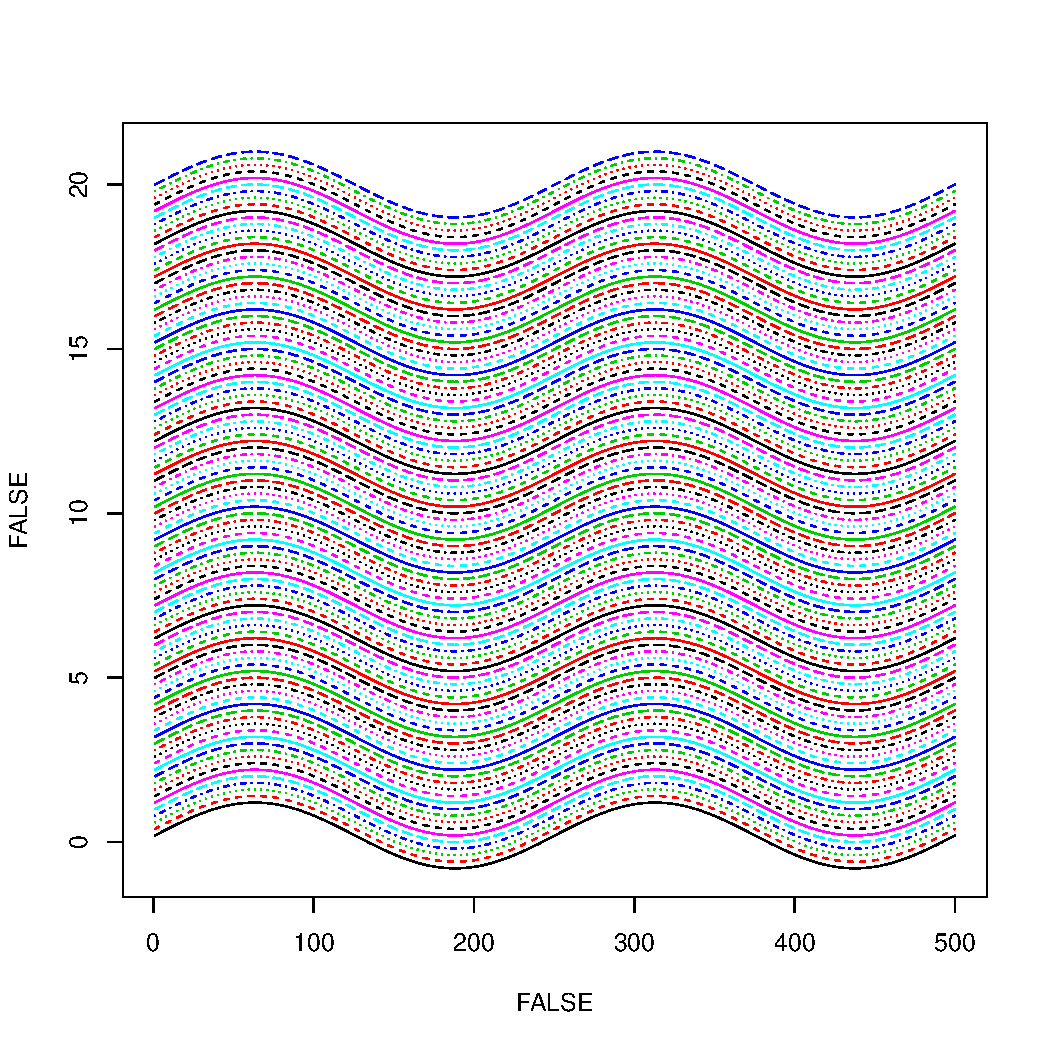
\includegraphics[scale=0.25]{img/I_tower.pdf}
 \end{minipage}
 \hspace{0.3cm}
 \begin{minipage}{0.55\textwidth}
  \centering 
  \includegraphics[scale=0.5]{img/tower.pdf}
 \end{minipage}
\end{figure}

\textbf{Nota}:
Il dataset usato per il test \`e \texttt{synthetic/towerSine}.

\end{frame}

%%%%%%%%%%%%%%%%%%%%%%%%%%%%%%%%%%%%%%%%

\subsection{Outlier}

%%%%%%%%%%%%%%%%%%%%%%%%%%%%%%%%%%%%%%%%
\begin{frame}
 \frametitle{Esempio: Outlier}
Con questo esempio si studia la capacit\`a delle profondit\`a di cogliere le curve \emph{outlier} di un dataset.
Il dataset artificiale usato presenta 10 outliers di ampiezza, le cui profondit\`a sono minori di quelle degli altri dati.

\begin{figure}
 \begin{minipage}{0.4\textwidth}
  \centering
  \includegraphics[scale=0.25]{img/I_outlier.pdf}
 \end{minipage}
\hspace{0.3cm}
  \begin{minipage}{0.55\textwidth}
   \centering
  \includegraphics[scale=0.5]{img/outlier.pdf}
  \end{minipage}
\end{figure}

\textbf{Nota}:
Il dataset usato per il test \`e \texttt{synthetic/outlierSine}.



\end{frame}

%%%%%%%%%%%%%%%%%%%%%%%%%%%%%%%%%%%%%%%%

\subsection{Boxplot}

%%%%%%%%%%%%%%%%%%%%%%%%%%%%%%%%%%%%%%%%
\begin{frame}
\frametitle{Esempio: Boxplot Funzionale}
Con le profondit\`a appena calcolate \`e possibile costruire dei boxplot funzionali, generalizzazione di quelli del caso standard numerico unidimensionale.\\
La determinazione di outliers \`e importante per irrobustire un dataset o determinare delle anormalit\`a morfologiche.

\begin{figure}
 \centering
\includegraphics[scale=0.2]{img/fbplot.pdf}
\end{figure}
Vengono marcati come outliers i segnali che eccedono, in almeno una delle dimensioni e in almeno un istante $t \in I$, da $1.5$-volte l'inviluppo della \emph{regione centrale}, cio\`e il
$50\%$ dei dati pi\`u profondi.

\end{frame}
%%%%%%%%%%%%%%%%%%%%%%%%%%%%%%%%%%%%%%%%
\begin{frame}

\begin{center}
\rule{5cm}{2pt}\\
\Large Grazie per l'attenzione.\\
\rule{5cm}{2pt}\\
\end{center}
 
\end{frame}


%%%%%%%%%%%%%%%%%%%%%%%%%%%%%%%%%%%%%%%%

\end{document}
